\documentclass[conference]{IEEEtran}
\IEEEoverridecommandlockouts

\usepackage{cite}
\usepackage{amsmath,amssymb,amsfonts}
\usepackage{algorithmic}
\usepackage{graphicx}
\usepackage{textcomp}
\usepackage{xcolor}
\usepackage{algorithm}
\usepackage{algorithmic}

\def\BibTeX{{\rm B\kern-.05em{\sc i\kern-.025em b}\kern-.08em
    T\kern-.1667em\lower.7ex\hbox{E}\kern-.125emX}}

\begin{document}

\title{ECE 276B Project 1: Dynamic Programming for Policy Learning in MiniGrid Environments}
%{\footnotesize \textsuperscript{*}Note: Sub-titles are not captured in Xplore and should not be used}}

\author{\IEEEauthorblockN{Iulia Rusu}
\IEEEauthorblockA{\textit{UC San Diego}\\
San Diego, CA}}

\maketitle

\begin{IEEEkeywords}
dynamic programming, MiniGrid, navigation, MDP, policy
\end{IEEEkeywords}

\section{Introduction}
We are given a series of MiniGrid maze environments, these are grid-based worlds comprised of obstacles in the form of walls,
doors placed in various locations, and keys which can be used to open closed doors. An agent is placed in said environment and needs to navigate the maze
to a goal location. We analyze this problem through the lense of a control setting, in which an agent must learn a policy, $\pi$, a distribution over states, $x \in X$ and actions $u \in U$ 
that minimizes overall cost to navigate these obstacles efficiently and reach a goal.
We explore this in two settings: part A) one in which we are given 8 maze environments fully known before hand, and Part B) one in which
we are given a selection of random environments. To derive the appropriate action sequences for parts A and B
we create 8 unique policies for part a, and one general policy that works for all the environments in part b.  
This type of problem includes challenges such as navigation, object manipulation, and exploration, 
all of which are important features of successful problem solving in robotics. Our approach at a high level
relies on using the Dynamic Programming algorithm, with which we solve for value function and policy, which
allows the agent to navigate each problem setting successfully.

\section{Problem Statement}
\subsection{MDP}
We define our problem in the context of a Markov Decision Process, or MDP, in the finite horizon setting. An MDP is a mathematical
model for sequential decision-making in which outcomes can be stochastic. The MDP is a time dependent process, characterized by the following tuple:

\begin{align}
(\mathcal{X}, \mathcal{U}, p_0,p_f, T, \ell, q, \gamma)
\end{align}
 
These are the state space, control space (or action) space, initial state , a conditional pdf, time horizon, stage cost, terminal cost, and discount factor.

We define control policy $\pi$ as a function that maps a time step $t \in T$ and a state $x \in X$ to a control input $u \in U$. There is a cost $\ell(x, u)$ associated with taking an action at a 
given state. We can calculate the expected cumulative cost of a policy $\pi$ applied to an MDP starting at an initial state $x$ at a given time $t$. This is called the value funtion $V_t^\pi(x)$
and it is defined as follows:

\begin{align}
V^\pi_t(\mathbf{x}) &= \mathbb{E}\left[q(\mathbf{x}_T) + \sum_{\tau=t}^{T-1} \ell(\mathbf{x}_\tau, \pi_\tau(\mathbf{x}_\tau)) \,\Big|\, \mathbf{x}_t = \mathbf{x}\right]
\end{align}

The parts of the MDP defined the same in both part A and part B:
$\mathcal{U}$ = {MF, TL, TR, PK, UD} The 5 actions are always the same: Move Forward, Turn Left, Turn Right, Pickup Key, Unlock Door.
$q(x) = 0$ if the state is a goal.
$\ell(x,u) = 1$ is the stage cost for all actions in all states except the terminal.
$T = \text{width} \times \text{height}$ The time horizon is calculated depending on the size of the environment. The transition matrix,
$p_f(\cdot \mid \mathbf{x}_t, \pi_t(\mathbf{x}_t))$ is calculated deterministically, action transitions are deterministic, if moving from one state to the next via an 
action, it has p =1 of happening.
$\gamma = 1$ The discount factor is always 1.

The differencs are in $x$ and $p_0$ between part A and Part B. In part A:
\begin{align}
x = [\text{x position}, \text{y position}, \text{direction}, \text{key state}, \text{door state}]
\end{align}

Key state refers to if the agent is carrying a key or not, and door state
refers to if the only door is open or closed, these are both binary. X and y position are dependent on the dimensions of width and height or the environment, and there are 4 directions for facing (north,
south, east, or west).
$p_0$ varies depending on the starting position of the agent in each of the 8 environments.

State definition in part B is an expanded version of the previous state, this time including key location and goal location:
\begin{align}
x = [&\text{x pos}, \text{y pos}, \text{direction}, \text{key state},\nonumber\\
     &\text{door1 state}, \text{door2 state}, \text{key loc}, \text{goal loc}]
\end{align}


Key position is always 1 of 3 options, so is goal positions. And the environments now have 2 doors.
$p_0$ is always (4, 8) facing up, and the state scalar for this is computed according to these specifications.


\subsection{Dynamic Programming}
We chose to solve both part A and part B by approaching the navigation problems using Dynamic Programming (DP). 
Dynamic Programming is an algorithm that allows one to solve optimization problems by computing an optimal value function
$V_0^{*}(x_0)$:
\begin{align}
V^*_0(\mathbf{x}_0) &= \min_{\pi} V^\pi_0(\mathbf{x}_0)
\end{align}
and an optimal policy $\pi^*$:
\begin{align}
\pi^* \in \arg\min_{\pi} V^\pi_0(\mathbf{x}_0)
\end{align}   

The algorithm does this by going backwards in time, starting from the goal. Time convention is discrete from $t_0,..., T$. After it defines all the components in the MDP tuple, it computes the value function for all terminal states $x_T$,
for the final time step this is just known as $q(x)$ the terminal cost. From there on out in loops backwards in time from $T-1$ to $t_0$ and computes the Q-values of each
$x$ and $u$ pair, the Q-value computation involves knowing the stage cost $\ell(x,u)$ of the state action pair, and the expectation over value functions of the next state, given
we know the probability of reaching that next state, given the current state and action is given by $p_f$. We derive the value function the the state at the time, by taking the 
value in the Q-table taken from the action that minimizes the Q-table row for that state. And the policy at that time, is the action itself. The algorithm is as follows:

\begin{algorithm}
\caption{Dynamic Programming}
\begin{algorithmic}[1]
\STATE \textbf{Input:} MDP $(\mathcal{X}, \mathcal{U}, p_0, p_f, T, \ell, q, \gamma)$
\STATE $V_T(x) = q(x), \quad \forall x \in \mathcal{X}$
\FOR{$t = (T-1) \ldots 0$}
    \STATE $Q_t(x, u) = \ell(x, u) + \gamma \mathbb{E}_{x' \sim p_f(\cdot|x,u)}[V_{t+1}(x')], \quad \forall x \in \mathcal{X}, u \in \mathcal{U}(x)$
    \STATE $V_t(x) = \min_{u \in \mathcal{U}(x)} Q_t(x, u), \quad \forall x \in \mathcal{X}$
    \STATE $\pi_t(x) = \arg\min_{u \in \mathcal{U}(x)} Q_t(x, u), \quad \forall x \in \mathcal{X}$
\ENDFOR
\RETURN policy $\pi_{0:T-1}$ and value function $V_0$
\end{algorithmic}
\end{algorithm}


\section{Technical Approach}
In the code we use two different implementations of the Dynamic Programming algorithm one for Part A and one for Part B.

\subsection{Part A}
Grid sizes for part A range from 5x5 to 8x8. There are 4 possible directions to face, north, south , east, or west. The key can be in any location. Walls are not walkable, 
neither are closed doors.
In order to pick up a key, the agent needs to be in a cell facing the cell with the key in it, and choose the PK action.   

Before the DP is ran the $P_f$ matrix is calculated by creating all possible combinations of state. This is done for each of the 8 environments separately, because each one
has a different configuration of walls, size and goal.
A dictionary for each environment called $Pf$ is initiated. There are nested for loops over each part of the definition of the state:
a for loop over $\text{range}(x)$, for loop over $\text{range}(y)$, 
The inner layer is a for loop over the 5 actions. Before this we skip over states that are not allowed to exist, for example: any x,y combinations that land on unwalkable surface,
or if x,y,dir is a goal location. The state $x \in \mathcal{X}$ is a combination of the following factors: x position, y position, direction, key state, door state.
Key state and door state are boolean values, 0 for does not have key, 1 for has key, and 0 for closed door, 1 for open door. If a state is allowed to be in the environment 
it is calculated as a scaler using the following heuristic: 
\begin{align}
s = x + W \cdot (y + H \cdot (\text{dir} + 4 \cdot (\text{key state} + 2 \cdot \text{door state})))
\end{align}

And if it is not in $P_f$ then it is added.
Then we begin perform each action to the according to the transition rules. We don't use the actual environment to perform the action, but use a dictionary to calculate the 
dx and dy values to go from one position to the next, or we turn the agent by switching the direction value using a module system.
There are caveats such as, if an action such as move forward takes the agent to a wall, the perimeter of the maze, or a closed door, these positions are unwalkable, 
and therefore $\text{next state} = \text{state}$. 
If the action transitions us into a new next state we use the same equation as above to generate the scalar value for it, replacing the changed variables.

Each entry in this completed dictionary is index as such $Pf[\text{state}][\text{action}] = [\text{next state}, \text{cost}]$. 
Cost for everything in the dictionary is always 1.

Then we run our DP algorithm, the code for this is structured in for loops and runs closely to the algorithm outlined in the Problem Statement.
Before we run the algorithm, we generate an array for the value function, the size of all state (including not allowed ones). This array we fill with np.inf.
Then we find the state values of the goal position, and fill those positions in the V array with 0, this is the terminal cost for all states, and V becomes our $V_T$.
Then we start a loop backwards in time going from $[T-1, 0]$ in increments of 1. In the loop we create a fresh Q-table, an array the size of states x actions,
for all states for all actions we compute the Q-value of T-1 in the first iteration, and the $V'$ is our computed $V_T$. We then compute the new $V$ using the min of the Q-table.
The premade $P_f$ matrix is used to calculate the expectation value in the Q-table. The probability of the next state is always 1.
In each step of the algorithm we override our V array, so we do not store the intermittent time steps. Using the $V_t$ we compute the policy, an array that is time x state.
In each column of the array the optimal action at that state in time is stored.

So at a high level, we use three main functions: \texttt{gen\_Pf} , \texttt{dynamic\_programming} and \texttt{run\_policy}. We run the $Pf$ generating function for each of the 8 environments and pass the resulting transition dictionary into a separate instance of the DP function. 
The DP returns a time-indexed policy $\pi[t, s]$ over all valid states. To generate the action sequence, we compute the initial state scalar from the agent's starting 
position, direction, key state, and door state. We then run a forward simulation: at each timestep $t$, we look up $\pi[t, \text{state}]$ to get the action, append it to 
the sequence, and use $Pf[\text{state}][\text{action}]$ to transition to the next state. The simulation terminates when the agent's $(x, y)$ position matches the goal 
position. This sequence we input into the gif making function, and use this to create trajectory plots.


\subsection{Part B}
The implementation of DP for Part B is similar to part A, except we use an expanded definition for state (which increases the whole state space), which includes
goal position and key position as additional factors. 

\begin{multline}
s = x + W(y + H(\text{dir} + 4(\text{key state} \\
+ 2(\text{door1 state} + 2(\text{door2 state} + 2(\text{key idx} + 3 \cdot \text{goal idx}))))))
\end{multline}

There are three different key and goal locations. The implementation creates just one $Pf$ dictionary, as this encompasses all possible scenarios found within the 36 random envs. Because the walls and the door locations are the same
for all 36, these positions were hard-coded, so was the state size (10 x 10). Therefore there was no need to use and interact with any specific env when looking at action related
state transitions. The for-loop system was larger and included 2 separate door booleans ( door 1 and door 2), and a for loop over all possible goal locations, and a for loop
over all possible key locations.

The high-level implementation in the code included a \texttt{gen\_Pf} , \texttt{dynamic\_programming} and \texttt{run\_policy} functions.  

When loading the two environments for the two different cases, the loading functions are different. But we still used \texttt{load\_env} for our random environments. It was easier to
load each separate environment in a for loop over a range of values, the \texttt{load\_env} function only works for 1 door, since random environments had two doors, it still worked
but in the \texttt{run\_policy} function for the random case, we had to hard code the door positions.

\section{Results}
In part A there are 8 different maze environments, each consisting of a single closed door, and a single key. The agent's starting
position on the x,y grid and direction is different in each of these. We used a finite horizon for both settings. In Fig. 1 we display all 8 of the environments with the agent shown
as a red triangle and the goal location shown as a green square. As mentioned, walls are not walkable, neither are closed doors. The agent needs to open a door while carrying a key in order
to walk through it.
In order to pick up a key, the agent needs to be in a cell facing the cell with the key in it, and choose the PK action.   

We see that our DP policy implementation was successful in Figure 1. The red line shows the trajectory of the agent as it moves through the space. Unfortunately the turning and
key picking up actions are not visible as this just shows the movement, a clearer live version is found in the gifs of this report. We note that the trajectories are tight,
the agents spends minimal steps in completing each objective.

In terms of computational time, it took 0.9 seconds to run the whole dataset.

\begin{figure}[htbp]
\centerline{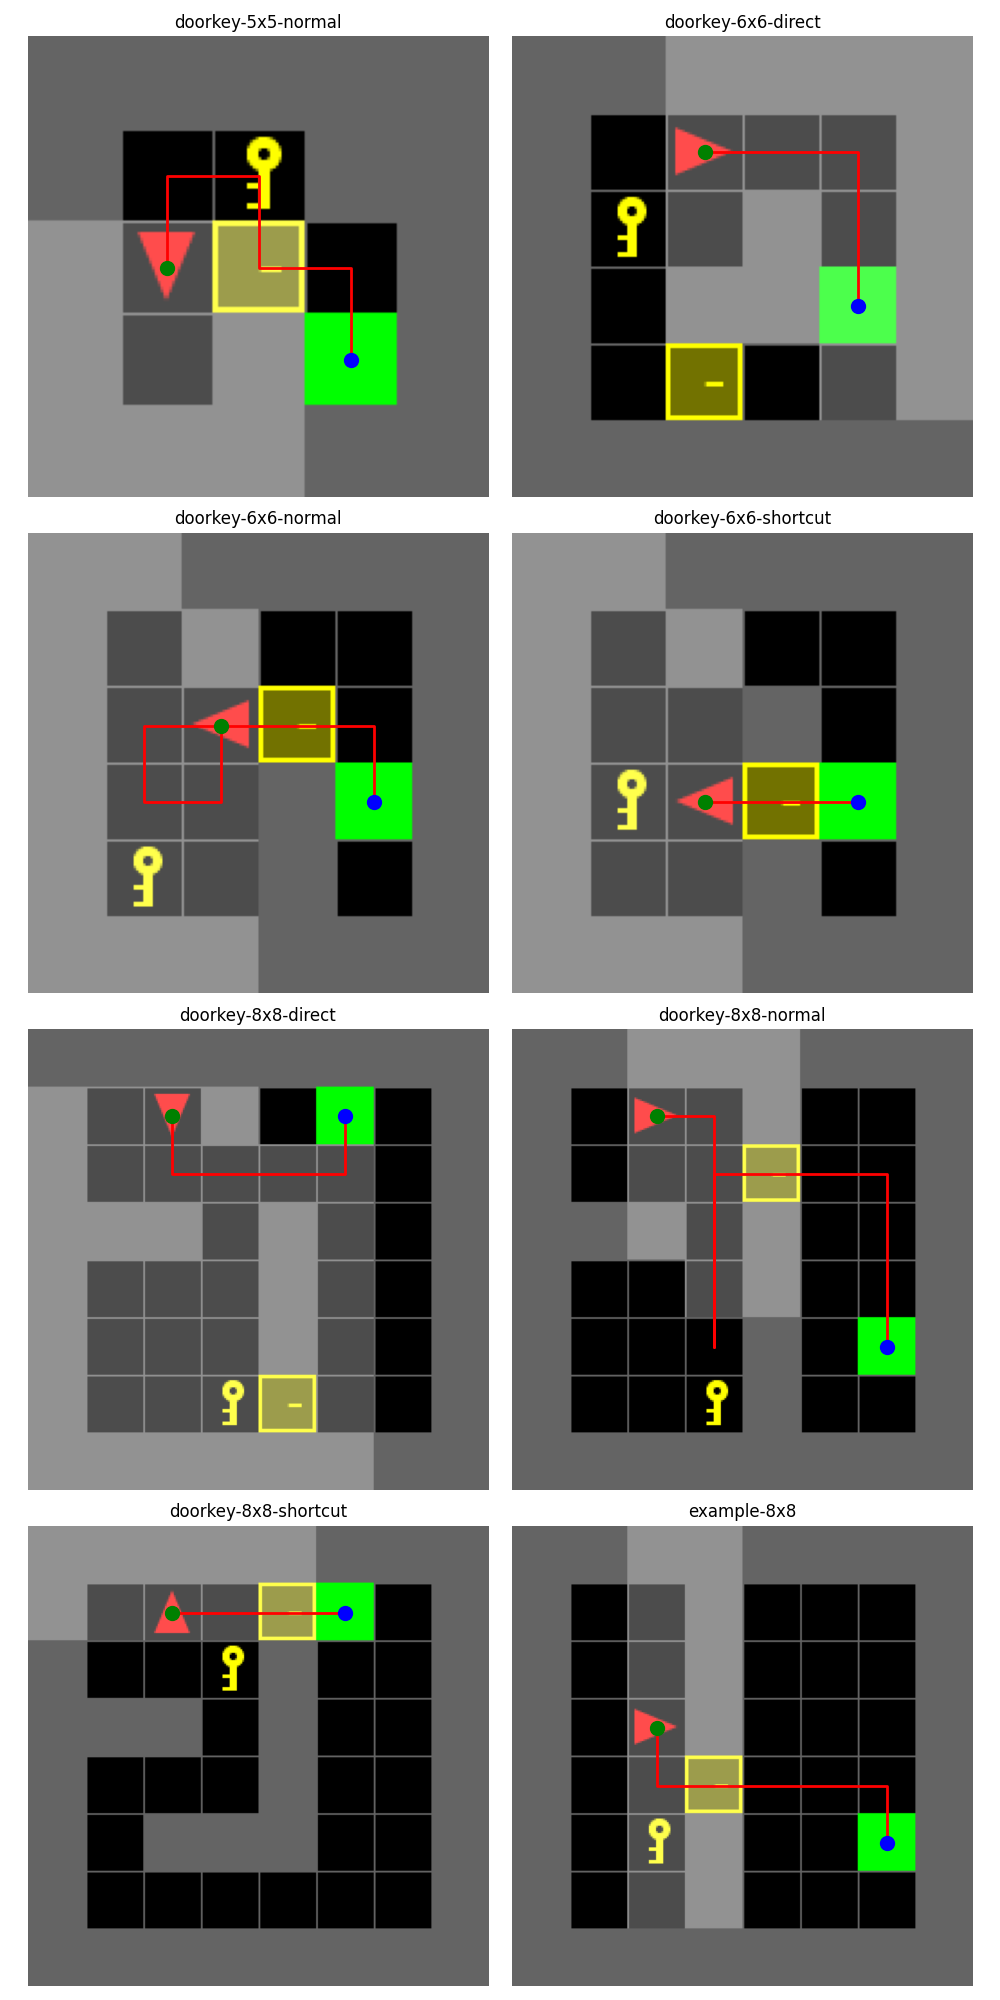
\includegraphics[width=\columnwidth]{./starter_code/gif/all_envs.png}}
\caption{Part A, policy evaluation on eight MiniGrid environments.}
\label{fig}
\end{figure}

In the second part of the project, we report the outcome of our policy on 36 different environments. In each of the random environments we are only given the following constants:
walls are always at the same positons on the grid, there are always 2 doors, but the state of each is random, and the agent is always located in the same cell facing the same direction.

Once more we are limited to only visualizing the red trajectory of the agent in each environment, so we may not see the direction turns and the action of picking up the key
has to be inferred. The data in the gifs demonstrates that all 36 environments were successfully solved. The total computation time for this was 9 seconds (including gif generation).

\begin{figure}[htbp]
\centerline{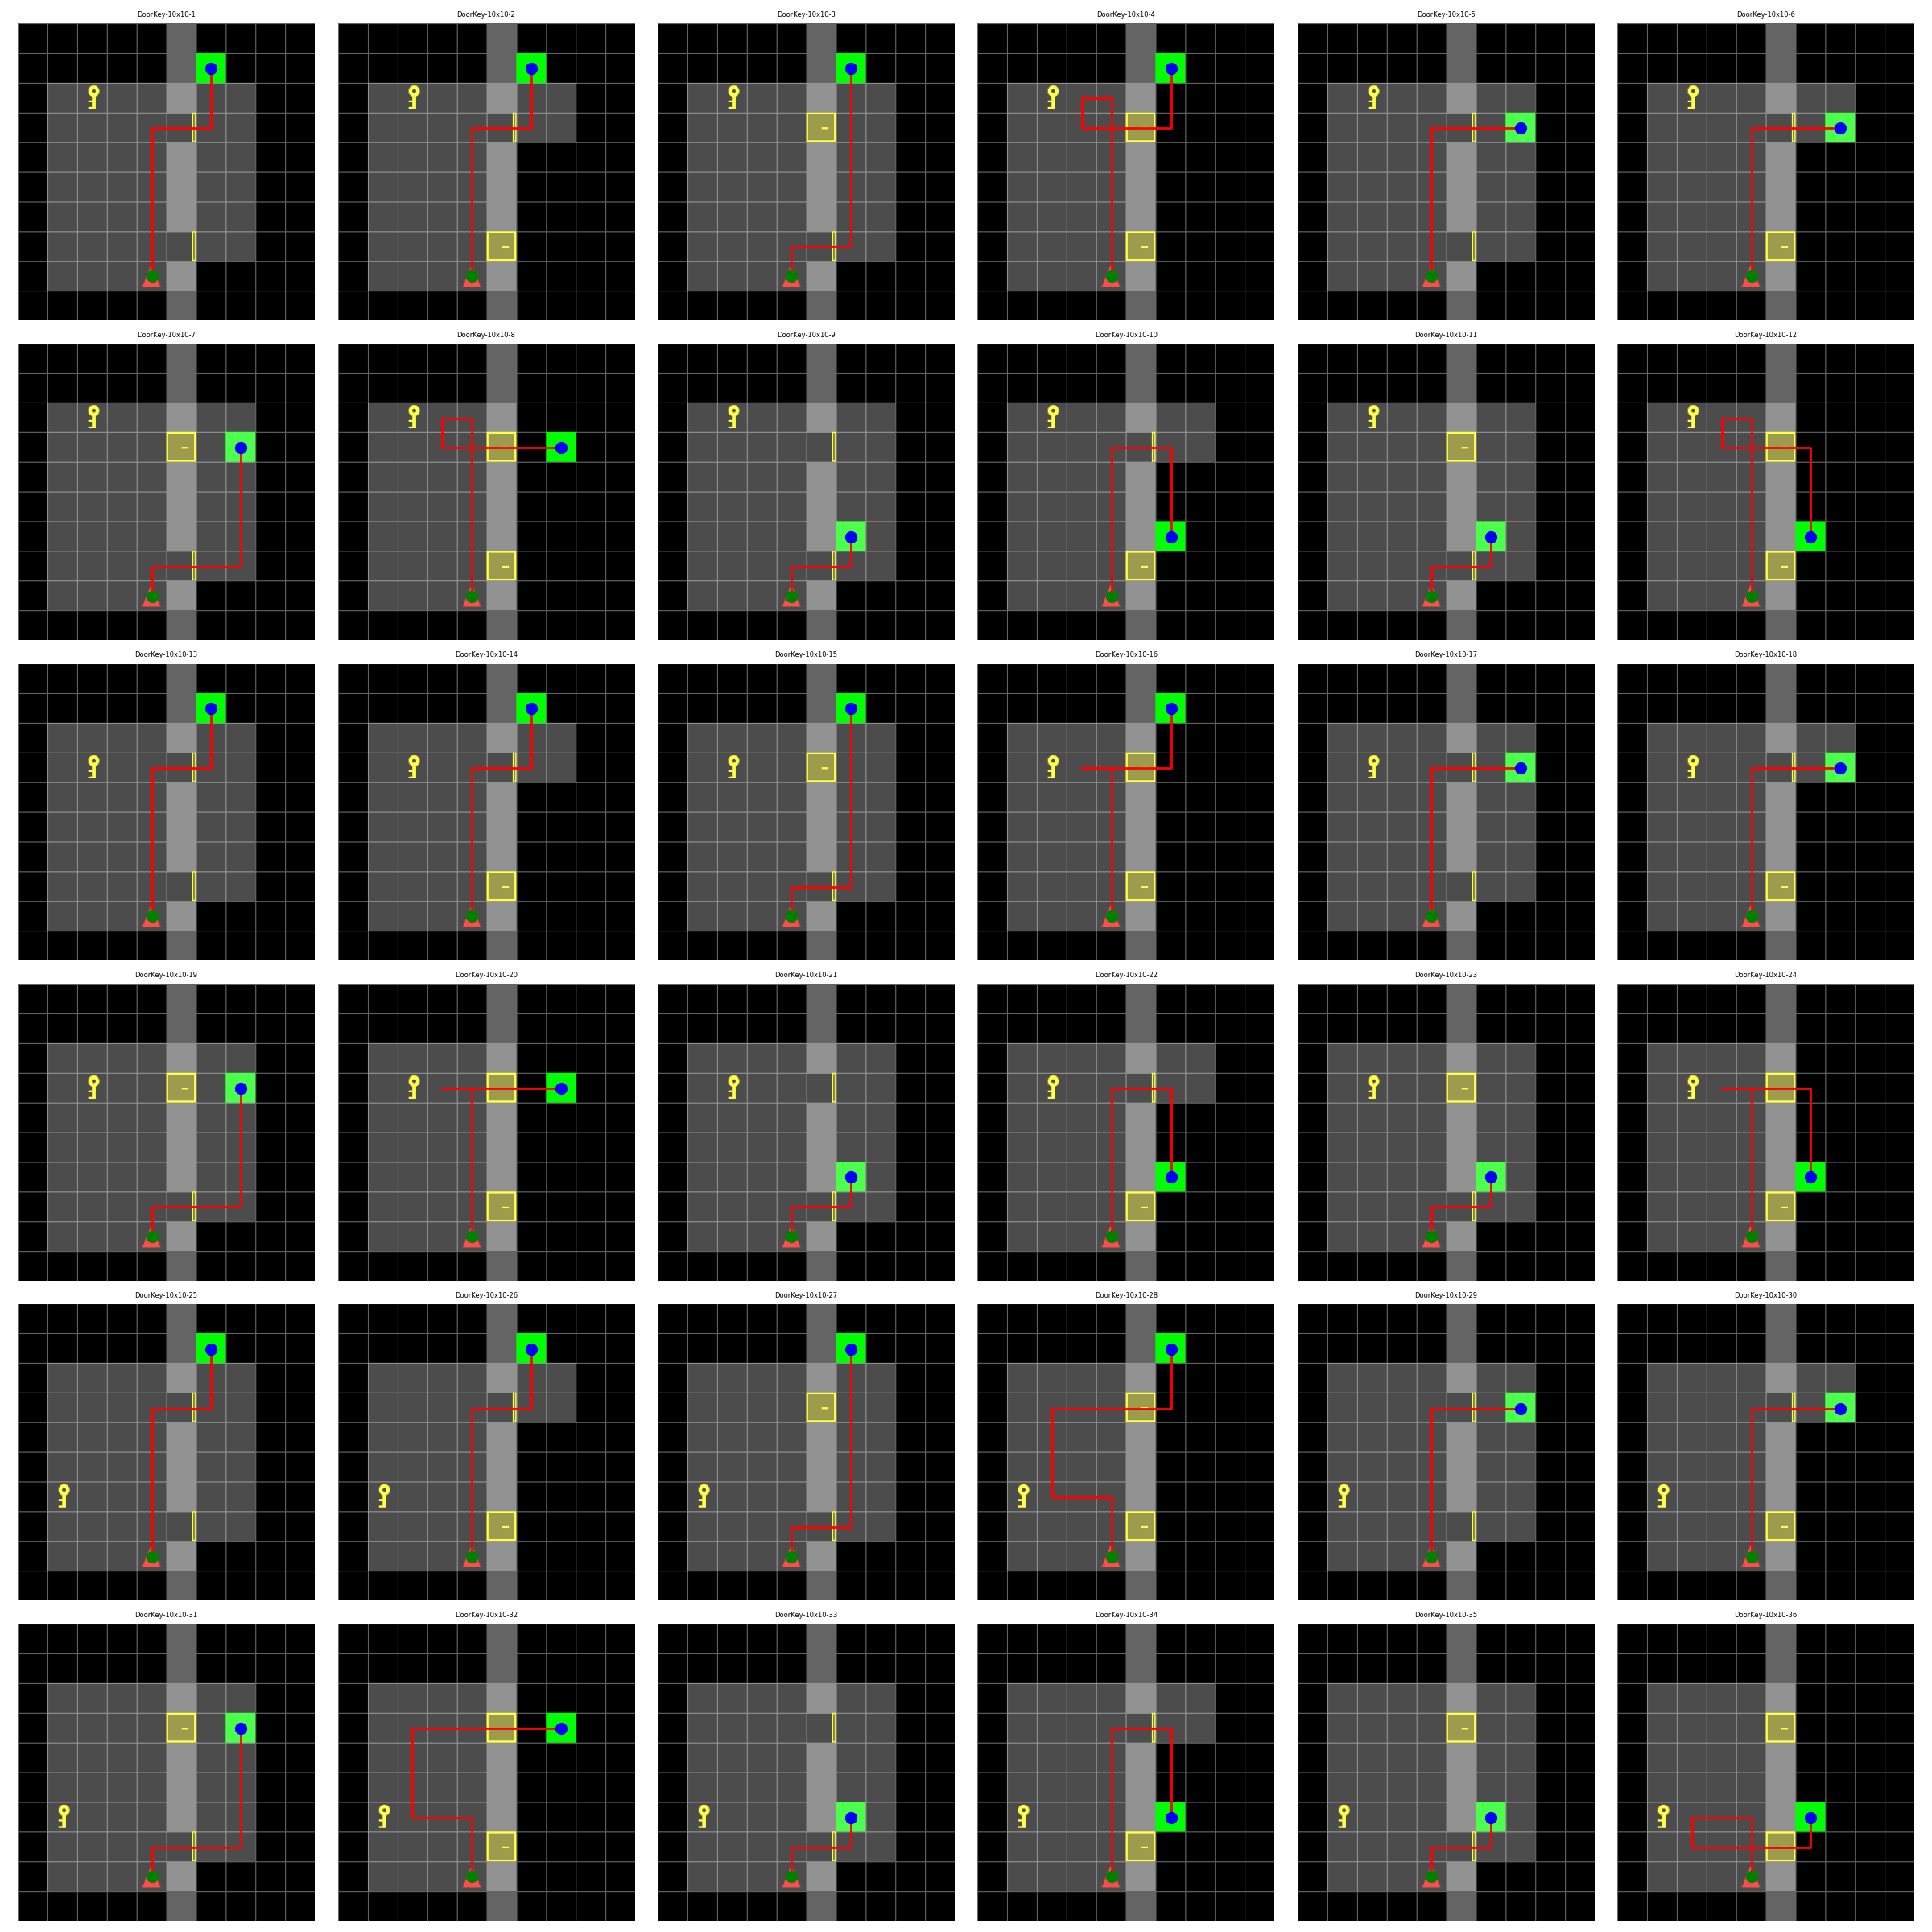
\includegraphics[width=\columnwidth]{./starter_code/gif/all_rand_envs.png}}
\caption{Part B, 36 random environments navigated using one policy.}
\label{fig}
\end{figure}


In practice $P_f$ was difficult to set up. The implementation of DP starts with finding goal states in the $p_f$ dictionary, happens using loops with the full range of width and length 
of the environment, but a vast majority of these combinations are not present in the dictionary. So a more efficient way of both creating $p_f$ and also indexing items in it, would make the 
code run faster. There could be a speed up in computation by providing a cleaner estimate of T. T was set by using the total number of grid cells, assuming the maximum longest path is the full size 
of the grid space, but still include unwalkable objects. The value function and policy are still optimized, but the algorithm might run longer than necessary. 
The gamma parameter was set to 1 for both Parts A and B. However it can in principle be changed to values <1 for greedier early behavior.

Overall the algorithm was implemented successfully in both cases as evident by the trajectories in Fig.1 and Fig.2. We include the gifs of all environment implementations and
the code in addition to this write-up.


\bibliographystyle{IEEEtran}

\bibliography{references}


\end{document}
